\onehalfspacing
\label{chapter3}
\section{A Working Definition of Flow}

In comparison to its conceptual counterpart the beat, flow resists a clear definition in
academic and technical discourse. While there seems to be some agreement that the beat is
comprised of musically-distinct layers looping throughout a piece, definitions of flow 
range from anywhere as specific as ``simply the rhythms and rhymes [a hip-hop song] 
contains''\footnote{
    \autocite[63]{pauledwardsHowRapArt2009}. While Edwards' statement comes within the 
    context of an instruction on rapping (and therefore his reductiveness may be 
    pedagogically useful), this attitude toward flow is implied by music academics who 
    transcribe flow primarily on one line of staff notation; such transcriptions implicitly
    show flow as something existing within a fixed (or indiscernible) pitch space, with 
    unambiguous, highly discernible rhythms.} 
to as wide-ranging as ``all of the rhythmical and articulative features of an emcee's 
delivery of the lyrics.''\footnote{
    \cite{kyleadamsMetricalTechniquesFlow2009}.} 
Before I discuss the stylistic hallmarks of flow in underground hip-hop, I will ascertain
a definition of flow more broadly.

Consider, once more, Open Mike Eagle's characterization of his own relationship to MF 
DOOM's flow: that Eagle has to be careful with it because of how much time he has spent
`in DOOM's mind.''\footnote{
    \cite{estellecaswellRappingDeconstructedBest2016}. For my earlier discussion of this
    passage and its relationship to meditative listening,  see Section 
    \ref{listeningasmeditation}.} 
His relationship to DOOM's flow demonstrates the term encompasses more than rhythm and 
rhyme alone; by themselves, these elements do not account for flow being tied to an emcee's
specific or generic style. Flow, then, refers to something more than the manifestation of 
rhythm through an emcee's rhymes. At the same time, emcees describe flow as text contextualized
in music, drawing contrasts with non-musically-bounded poetry. The emcee Rakim coined a
definition of rap as ``rhythm and poetry,'' distinguishing between texts that can be rapped 
and texts as only poetry. Clarifying this distinction, the emcee Myka 9 of Freestyle Fellowship
offers: ``sometimes I might write a poem, a spoken-word poem, but then morph that into a rap
rhythmically.''\footnote{
    \autocite[63]{pauledwardsHowRapArt2009}.}
Myka 9's insight suggests a continuum for rapped text; it exists on a spectrum of text delivered
in musically-bounded ways and non-musically-bounded ways.\footnote{
    Interestingly, rapped verses can be and often are delivered on varying degrees of this
    spectrum. Mitchell Ohriner notes two distinct modes of delivery, which he calls speech-rhythmic
    and music-rhythmic, based on the degree of non-alignment between the musical meter and the 
    degree to which syllable onsets correspond to metrical positions (see 
    \cite{mitchellohrinerLyricRhythmNonalignment2019}.}
Emcees, therefore, have two concerns with flow: how a text is structured and how it is performed.

The distinction between the rap's structure as text and its performance as music is foundational
to my interrogation of flow in this chapter. I believe the techniques underground emcees employ 
when rapping can be divided into  categories I refer to as \emph{structural} and \emph{performance}
techniques. Structural techniques deal primarily with rap as text, considering its syntactic 
elements with primacy over their manifestation in the musical object. By contrast, performance
techniques focus on rap as music, considering the means by which an emcee expresses the structures
they contrive; this also encapsulates the decisions they make when treating the voice as an object
within a digital recording. With these categories, I aim to examine how, as Mitchell Ohriner claims,
flow ``encompasses phrasing, rhythm, meter, accent, patterning, and groove, not to mention the 
relations among these parameters.''\footnote{
    \autocite[28]{mitchellohrinerFlowRhythmicVoice2019}.}

\section{Chapter Overview and Definitions}

In this chapter, I examine four techniques that underground emcees employ in structuring and
performing their flow; I argue that, like producers, their choice to use these techniques reaches
listeners as underground. The techniques I define below do not run the gamut but rather feature in
salient examples of the subgenre. My terms divide into subcategories of structural and performance
techniques, a distinction based on my preceding discussion of flow. When the underground emcee 
inhabits the role of writer, they experiment with structuring techniques including \emph{pivot rhyme}
and \emph{closing fragmentation} to craft their verses. Stepping into the recording booth or onto 
the stage, the emcee shifts into their role as rapper and therefore draws on performance techniques
such as \emph{mimesis} and \emph{processing} to shape their vocal delivery. Each of these techniques
serves as the focus of one of the close-readings that follow, so I will clarify their functions 
before provide examples.

As a device for constructing a verse, a pivot rhyme allows an emcee to execute a shift in end rhyme;
it occurs when the concluding words of the previous bar link to text that falls within the first beat
of the next bar. In this instance, the rapper uses a word or phrase as the primary rhyming structure
a new textual unit. Often the emcee uses this instance as a way to play with audience expectation, 
taking the listener's focus on this pivot rhyme to link units together semantically.

Underground emcees employ closing fragmentation to mark the end of some sort of formal section. To
accomplish this, emcees write a full syntactic unit, usually falling spanning the space of one bar,
then signal a close through fragmenting and repeating the component elements of the phrase in a more
improvisatory and loosely-organized style of delivery. Fragmentation and repetition here do not 
function as they do in the construction of a hook; rather, they demonstrate to the listener that some
larger textual unit\textemdash a verse-part, verse, the song itself\textemdash is ending.

With performance techniques, underground emcees position their voice as a layer\emph{amongst} the rest
of the musical mix, rather than the principal element within it. In particular, the use of mimesis, or
stylizing vocal delivery to mimic other elements in the beat layer, draws attention to elements of the
beat, foregrounding their musicality. This promotes the other musical layer to the role of co-soloist
rather than accompanist, so that the listener focuses it equitably with the flow.

In music production, processing more refers to the manipulation of digital audio after it is recorded
through the use of equalization (EQ), compression, and reverb, but here I use it specifically to discuss
changes made to the the vocal signal as a form of electronic composition. Rappers use processing effects
like delay, distortion, and pitch transposition to alter the audio of their voice during or after
tracking it as a producer might with any other musical element; the result is vocals that function as 
\emph{sound} as much as they do text.\footnote{
    This definition encompasses vocal glitch, a parallel process to what occurs in the production of 
    the beat (see Section~\ref{glitch}.)}
Processing treats the voice as if it were any other musical layer and democratizes its position within
the mix overall.

%clearpage
\section{Structuring Techniques}
Transcribing flow demonstrates the limitations of staff notation, perhaps more transcribing any other
musical element in hip-hop. Throughout this project, my dedication to standard notation transcriptions
arises from my desire to emulate what Kofi Agawu conceptualizes as a ``post  colonial transcription,''
one based in an ``ideology of sameness so that\textellipsis we can gain a better view of 
difference.''\footnote{
    \autocite[67]{kofiagawuInventionAfricanRhythm2003}. Agawu's chapter traces a history of 
    non-African scholars transcribing Northern Ewe drumming in a way that both essentializes
    and exoticizes African music as primarily rhythmic and therefore fundamentally different
    from Western approaches to music making. Although I do not wish to employ colonization 
    uncritically as a metaphor for music theory's relationship to hip-hop, I do believe that
    the same essentializing and exoticizing tendencies would manifest if I were to completely
    avoid standard notation for this repertory.}
However, my approach to transcription thus far has yet to factor in another point Agawu makes: no
singular mode of representation can sufficiently convey the totality of a listening 
experience.\footnote{
    \autocite[187]{kofiagawuAfricanRhythmNorthern1995}.}
In dealing with flow as a textual structure independent from its musical manifestation, 
I opt to use non standard representation of the music by transcribing using Ohriner's $modulo$ 16
grid transcriptions.\footnote{
    Ohriner overviews his system and details his justification for the method in 
    \autocite[xxviii--xl and 7--9]{mitchellohrinerFlowRhythmicVoice2019}, respectively.}

Ohriner's transcription method simplifies elements that become problematic when transcribing flow
in standard notation. His 16-point grid for a bar avoids proliferate use of eighth, sixteenth, and
thirty-second notes, not to mention syncopation between them. His method simplifies naming structure
by labeling  each metric position with a number from 0--15; one can more succinctly communicate a 
syllable landing on ``the third sixteenth note of beat 3'' as position 10, for instance. Lastly, 
Ohriner's system does not force a transcriber to choose fixed metrical positions in the same way
standard notation and adaptations of the Time Unit Box System (TUBS) for flow do; if a syllable 
onset occurs slightly before the beat, one simply moves the corresponding circle. Although vocal
groove and non-alignment with the beat's projected meter is not a focus in this chapter, the ability
for a system to adapt between quantized and non-quantized rhythms is foundational to being able to
transcribe flow.

\phantomsection
\subsection*{\centering Madvillain's ``Great Day''}
\addcontentsline{toc}{subsection}{Madvillain's ``Great Day''}

Madvillain, the title given to DOOM and Madlib's collaborations except for ``One Beer,'' looms large
in the world of underground hip-hop. One unrelenting focus of the accolades for  their 2004 double LP 
\textit{Madvillainy} is DOOM's flow: in the words of Ta-Nehisi Coates, ``[\textit{Madvillainy}'s] 
singular sound came mostly from [DOOM's] raspy baritone rendering a sort of nerdcore poetry.''\footnote{
    \cite{ta-nehisicoatesMaskDoomNonconformist2009}.}

This claim to DOOM's eccentricity finds purchase beyond the mythologizing in which Coates and much of 
the rest of the hip-hop community partake. Kyle Adams, for instance, notes that on ``All Caps'' both the
melodic samples (various portions of the main theme for the NBC crime drama \textit{Ironside}) and DOOM's
flow ``[seem] to float free of the meter, being only weakly tethered to it by the drum sample.''\footnote{
    \cite{kyleadamsMetricalTechniquesFlow2009}. What Adams notes about the \textit{Ironside} sample likely
    bolsters my claim that sample slippage is a frequently-employed technique in underground hip-hop 
    production, but it is not uniformly employed across Madlib's sampling practice (more on this below).}
Adams characterizes DOOM's flow in this way after examining the structure of its syntax; particularly, he
shows how rhymes in ``All Caps'' do not create metric regularity, and that syntactical units (Adams calls
them phrases) often cross metrical boundaries. DOOM's novel use metrical irregularity, per Adams, contributes
to the perception of DOOM as an underground rap artist.

While metrical ambiguity and enjambment may play a role in DOOM's sounding as underground on ``All Caps,''
I am hesitant to accept this as the whole picture of DOOM's alternative identity. A counterexample to the
techniques Adams accounts for on ``All Caps'' emerges from the track that immediately follows it on 
\textit{Madvillainy}\textemdash ``Great Day.'' The beat's primary melodic sample comes from ``How Do You 
Believe,'' an instrumental funk track by Stevie Wonder, released in 1968 under the alias Evits Rednow. Madlib
closely aligns the sampled elements (electric piano, harmonica, bass, and auxiliary percussion) with the drum
break he uses and marks out a hypermetric downbeat with a C-sharp minor gospel lick every fourth bar in the A
section.\footnote{
    This type of metric regularity also pervades ``One Beer,'' where the whole
    instrumental before the skit is sampled from one track by the funk band Cortex 
    (see Section~\ref{samplebased}.)}
    
    \begin{figure}[!t]
        \centering
        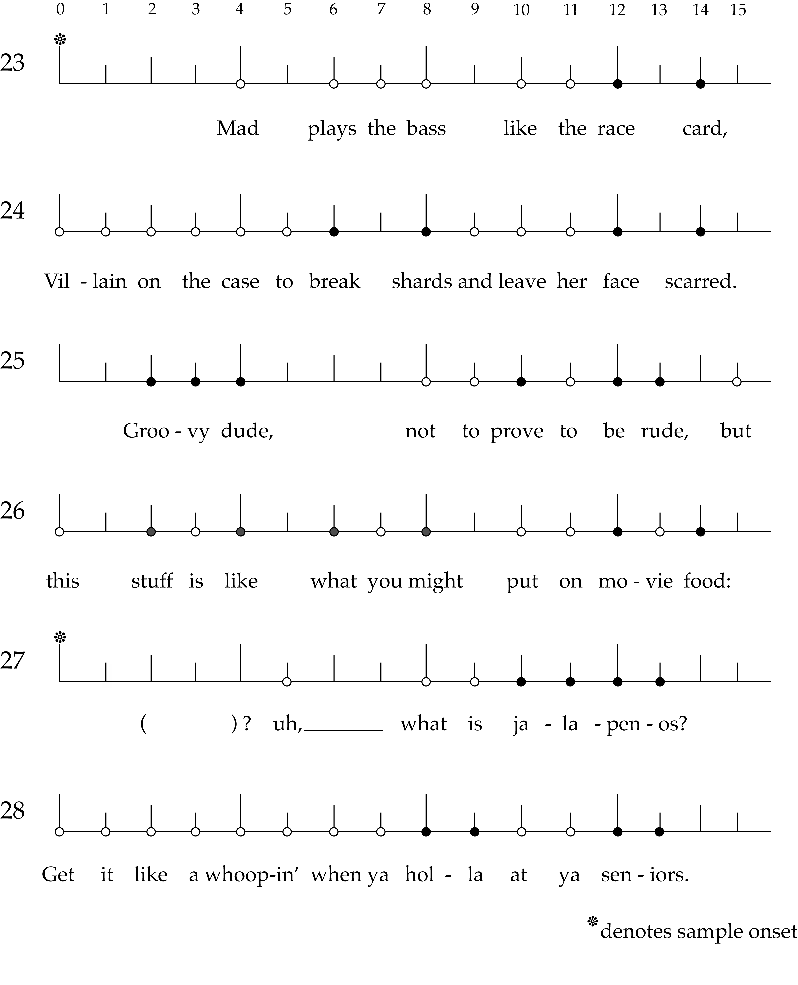
\includegraphics[width=0.8\textwidth]{images/figures/chp 03/059115greatdayavoidedpivot.pdf}
        \caption{Avoided pivot rhyme in Madvillain's ``Great Day,'' 0:59--1:15.}
        \label{fig:doomavoidedpiv}
    \end{figure}

Figure~\ref{fig:doomavoidedpiv} shows how DOOM, as might be expected, flows with a syntactic structure of a 
similar regularity. Entering after the downbeat where the sample loops, he raps: ``Mad plays the bass like the
race card, / Villain on the case to break shards and leave her face scarred.'' In these two bars, DOOM fits the
setup and punchline squarely within each barline, landing the two-syllable rhyme that closes each of them on 
positions 12 and 14. The internal rhyme in the second bar (``break shards'') occurs in a metrically weaker
position (6 to 8, as opposed to 4 to 6), but falls within what Ohriner refers to as the same durational segment
(in this case, a value of 2 on the grid). Rather than interrupting the sense of regularity in the flow, the 
internal rhyme in this bar creates an anticipation for the rhythmically ``restored'' position of the end rhyme.

Following the restoration, DOOM's flow becomes more syntacically and rhythmically complex, building up to
the four-bar loop of the sample. Bars 25 and 26 increase the number of syllable onsets from 18 to 22, as 
well as the  frequency, position, and syllable count of the rhymes. In the setup bar, DOOM creates an 
internal rhyme with ``Groovy dude'' and ``prove to  be rude,'' each fitting within a durational segment of
2 from positions 2--4 and 10--12, respectively. In the punchline, ``movie food'' once again restores the
metric position of the end rhyme, preceded by two softer, internal rhymes (``stuff is like'' with ``what
you might'' falling between 2--4 and 6--8). Despite the increase in internal complexity, the  syntactic 
structure of these bars maintains regularity: DOOM fits a sentence structured ``$x$, but $y$'' within the
same time span as the previous setup and punchline.
\clearpage

The structural regularity of the first four bars establishes a connection to the next four, two of which I
transcribed as a part of Figure~\ref{fig:doomavoidedpiv}. I perceive a semantic link in bars 26 and 27 that
DOOM to move on to a new structure but in the process invites me as a listener to imagine a pivot rhyme that
does not manifest. My expectation at the end  of bar 26 is that DOOM is going to rap about butter: not only 
because I put butter on ``movie food,'' but also because he has done so twice already on the album up to this
point.\footnote{
    DOOM refers to his ``buttery flow'' on ``Raid'' and Madlib's beats as ``so butter'' on ``All 
    Caps.''}
Somewhere in the first beat of bar 27, DOOM could mention butter and the word as a two-syllable rhyme that
sets up the end rhyme of the next quatrain. He, of course, thwarts this expectation, positing ``uh\textellipsis
what is jalapenos?'' as if  it were a botched  \textit{Jeopardy!} answer, linking an unexpected but semantically
related idea across bars 26 and 27. The bar instead opts for jalapenos as an end rhyme for the following quatrain.
With its final two syllables falling on positions 12 and 13, jalapenos ushers in a set of highly regular lines,
each ending with ``holla at ya  seniors,'' ``hashish fienda,'' and ``grass is greener'' in the same metric 
positions.

    \begin{figure}[!t]
        \centering
        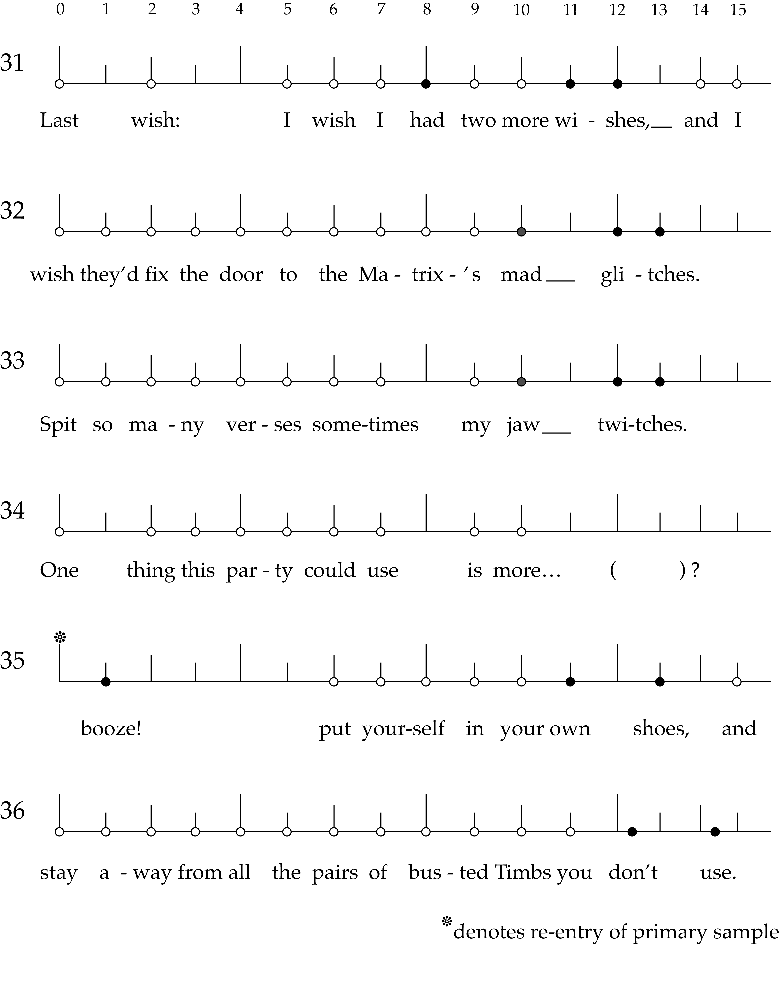
\includegraphics[width=0.8\textwidth]{images/figures/chp 03/121137greatdayachievedpivot.pdf}
        \caption{Pivot rhyme in Madvillain's ``Great Day,'' 1:21--1:37.}
        \label{fig:doomachievedpiv}
    \end{figure}

DOOM's avoided pivot rhyme and the next quatrain's regularity provide crucial context for a similar moment 
between bars 34 and 35, an instance where I do apply the term pivot rhyme. Figure~\ref{fig:doomachievedpiv}
overviews a third quatrain with a similarly regular structure. ``Wishes''  falls on positions 11 and 12, 
displaced 1 position forward from the ends of the two following  syntactic  closes: ``mad glitches'' and
``jaw twitches.'' DOOM's closely-related metric placement of the middle bars sets the listener up to hear:
``One thing this party could use is more\textellipsis booze.''And he makes that ellipsis audible! DOOM plays
on listener expectations not only concerning rhyme but also those concerning rap's ``topical stereotype:'' 
the trick of this moment is less his implication of the word ``bitches'' and more one's expectation that
he will say it.\footnote{
    My analysis of this moment varies slightly from Estelle Caswell's, who cites a \textit{Pitchfork} 
    reviewer's quotation that the ``hiliarity'' of this moment ensues from DOOM's non-sequitur (see
    \cite{estellecaswellRappingDeconstructedBest2016}).}
In effect, DOOM points the mic towards the listener at the end of the quatrain, asking them to examine
their own expectations.

DOOM's flow patterning and regulared syntactic structure lead to this moment; he crosses a barline, 
intentionally, yet again giving the listener a moment to expect one close to the phrase, before veering
off in another direction. As he continues on rhyming, this pivot on ``Great Day'' lingers because of its
play on expectation. Like an underground producer, DOOM has directly engaged a listener who has normative
expectations about a rhyme and content in a rap lyric, but his move away in this moment speaks to his
identity as an emcee.

%\clearpage
\phantomsection
\subsection*{\centering Armand Hammer and R.A.P. Ferreira's ``Dead Cars''}
\addcontentsline{toc}{subsection}{Armand Hammer and R.A.P. Ferreira's ``Dead Cars''}

Armand Hammer\textemdash a collaboration between billy woods and ELUCID\textemdash is a flagship act on
the roster of the New York based underground label Backwoodz Studioz. The track ``Dead Cars'' from the 
2019 LP \textit{Shrines} features production from Kenny Segal, as well as a feature verse from R.A.P. 
Ferreira\textemdash two premiere artists from Ruby Yacht, an underground hip-hop label for which Ferreira
serves as the owner-operator. Together, these artists work at the center of my conception of the underground,
and their techniques deeply inform my understanding of underground emceeing.

The track features several short verse-parts delivered by each of the emcees. Counting at 64 bpm, ELUCID, 
Ferreira, woods  rap for eight bars at a time, comparable to how jazz musicians may trade fours on a tune.
Ferreira's feature verse enters after ELUCID's second eight-bar section, accompanied by a drastic change 
in the musical texture. As Segal layers out the drum loop, he recomposes the original synth-texture chord
loop: a Fender Rhodes strikes chords on the downbeats and samples of reversed audio sound a melodic line
in between chord hits. Figure~\ref{fig:roryclosingfrag} transcribes the last six bars of Ferreira's verse, 
two bars prior to the drum's re-entry.

    \begin{figure}[!t]
        \centering
        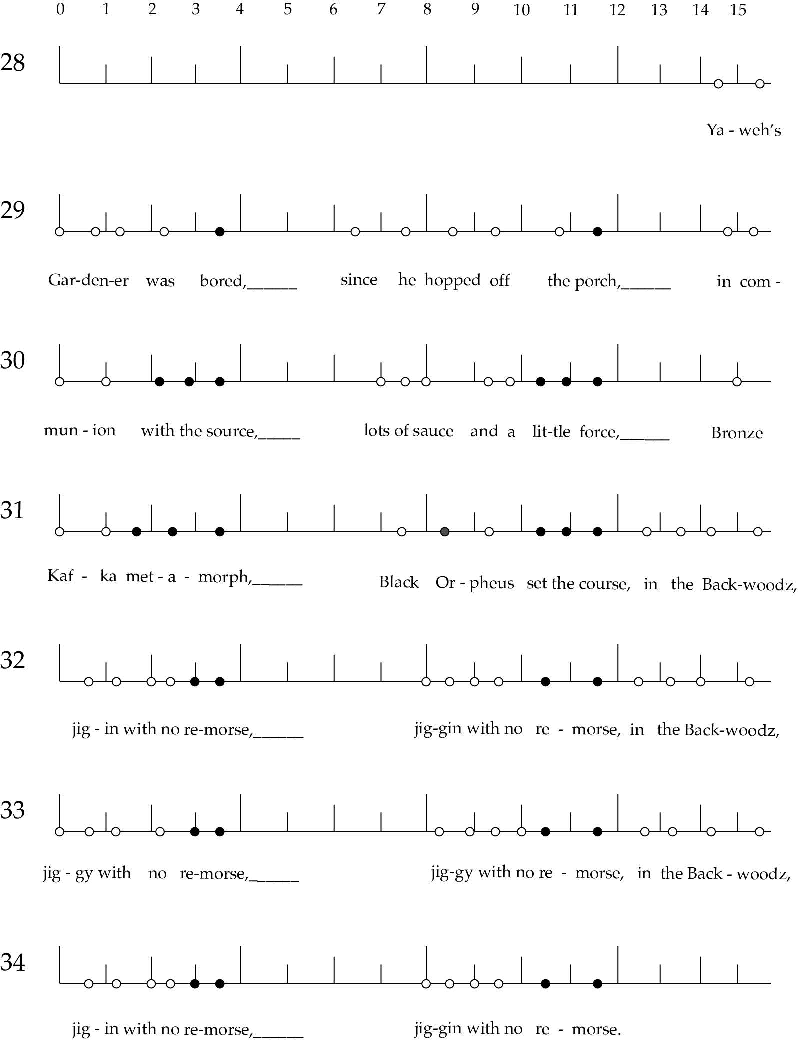
\includegraphics[width=0.8\textwidth]{images/figures/chp 03/144206deadcarsendfrag.pdf}
        \caption{Closing fragmentation in ``R.A.P. Ferreira's ``Dead Cars,'' 1:44--2:06.}
        \label{fig:roryclosingfrag}
    \end{figure}

Without drums demarcating a clear metrical hierarchy, Ferreira lets his text float around freely in 
micro-rhythmic space, but he uses rhyming syllables as an anchor for the more lax placement of the 
intervening text. He places his rhymes in slight anticipation of positions 4 and 12, where the snare
drum often hits in a drum loop.\footnote{
    According to Ohriner, orientation around these two beats is foundational to the 
    construction of the boom-bap texture pervasive in hip-hop beats (see his discussion
    of A\$AP Rocky's ``Purple Swag:  Chapter 2'' in 
    \autocite[18]{mitchellohrinerFlowRhythmicVoice2019}). My decision to mark out what 
    seems to be a slower, half-time tempo in ``Dead Cars'' is based on this orientation
    normalizes my hearing of the vocal sections as verse-parts rather than full verses.}
This rhyme structure may seem commonplace, but his choice to do so without snare hits helps to orient
a listener within the sparse musical texture. When, in bar 31, the drums do re-enter, Ferreira stops
rapping new text. Syntactically, his remaining four bars only rely on what I hear as two units: ``Bronze
Kafka metamorph, Black Orpheus set the course / in the Backwoodz, jiggin' with no remorse.''\footnote{
    My hearing of the first bar as a full syntactic unit is in part due to his rapping 
    of it within the space of one bar, but it has some semantic justification. I hear
    ``Bronze Kafka'' and ``Black Orpheus'' as two epithets the emcee gives 
    himself\textemdash the first a play on the author's name; the second, a nod to the
    1959 Brazilian film of the same name.}
The second of the two, a shoutout to his host emcees' label, becomes the textual focus of his shift into
a more improvisatory form of vocal delivery. Maintaining the rhythmic position of the final rhyming word
``remorse,'' Ferreira slightly alters his three repetitions of the phrase: the verb-form \textit{jiggin'}
becomes the adjective \textit{jiggy} as Ferreira shifts the metric placement of the first syllable to on
the beat in bar 32, position 1 and behind the beat in position 8. Before cycling back to a near direct 
repetition in bar 33, he accelerates ``Backwoodz'' from its original position, though still completing his
statement as a pickup to the next bar.

For a listener familiar with Ferreira's style, this textual unit serves as signposting that the verse is
coming to a close. When his text becomes fragmented, repetitive, and rhythmically varied, he is telling
a listener that he he about to finish rapping by employing closing fragmentation. This technique relates
to methods of delivering text that signal a change in formal sections theorized by Ben Duinker:
fragmentation and repetition can show that the rapper is no longer delivering a verse but instead either
a hook or a looser-organized vocal section.\footnote{
    \autocite[98--101]{benduinkerSongFormMainstreaming2020}. Duinker's definition of hook is 
    discussed on p.~\pageref{duinkerhookdef}. His ``looser-organized'' sections function like
    a catch all category; he includes ``ad-hoc, ametric vocals, skits, or\textellipsis [rapping]
    that doesn't function like a verse or hook'' as typical in this section-type.}
Constructed from examining form in mainstream hip-hop, Duinker's categories break down due to Ferreira's 
use of the technique within the verse. The rhyme scheme of the fragmented units matches that of the text
immediately preceding it (so, too, the metric placement of its rhymes). And though the text's semantics
may be construed as the kind of hype vocal that Duinker identifies, Ferreira locates them within a verse,
signalling its close. Closing fragmentation, then, becomes a valuable way to describe how an emcee deploys
fragmentation and repetition with a new categorical function.

In my listening, this technique most prominently occurs in Ferreira's catalog. His influence, however, can
be traced how other emcees use similar methods of sounding a close: members of the Ruby Yacht crew including
Pink Navel and S.AL occasionally use a repeated, closing bar when constructing their own rhymes, and on ``Dead
Cars,'' each of the verse-parts that precede Ferreira's end with closing fragmentation as well. In each case,
the use of of a comparable technique to signal a close rather than construct a new formal unit problematizes
typical formal boundaries in contemporary rap music. These moments change the way listeners engage with textual
repetition and therefore textual meaning, constructing a different type of identity narrative around the emcee.

%\clearpage
\section{Performance Techniques}
\phantomsection

An emcee's performance of flow demands a slightly different approach to the transcription of a musical object, 
one which can account more clearly for pitched elements and their interrelation with the beat. Ohriner's system
does not uniformly transcribe verses with pitch, but his more recent scholarship develops a contour-graph notation
to track changes in pitch broadly over the range of G2--G4 pitch-space.\footnote{
    \cite{mitchellohrinerAnalysingPitchContent2019}.}

My approach to representing pitch marks a point of departure from Ohriner's, likely due to conflicting
readings of the imperatives about transcription discussed in the prior section. He cites Agawu as 
justification for looking beyond the confines of standard notation. By contrast, I adamantly believe Agawu
suggests music theorists should use standard notation \textit{creatively} to articulate a complex picture of 
similarities and differences rap exhibits with a more-familiar repertory in our sphere of discourse. For this
reason, my transcriptions in this section harness standard notation diacritically, transcribing rap flows 
pitched in relation to themselves and other musical elements.\footnote{
    Such an approach to notation has precedence in \cite{robertkomanieckiVocalPitchRap2020}.}

\subsection*{\centering R.A.P. Ferreira's ``NONCIPHER''}
\addcontentsline{toc}{subsection}{R.A.P. Ferreira's ``NONCIPHER''}

If one were to look through R.A.P. Ferreira's catalog on any major streaming platform, they would guess that
the 2020 LP \textit{Purple Moonlight Pages} is an artistic debut, but this is not case. In reality, Ferreira's
career spans the entire preceding decade with a full catalog of releases under various monikers, the most 
prominent one being Milo. He ties the decision to switch to his own name closely to the concept of identity:
``my name is rory allen phillip ferreira. and after 9 years pro rapping i'm confident enuff to put it on what
i make. i never knew who milo was.''\footnote{
    See \href{https://twitter.com/yomilo/status/1134513544005849088?s=20\&t=nilLSy6nJ3-7JiVRfkP-Lw}
    {https://twitter.com/yomilo/status/1134513544005849088?s=20\&t=nilLSy6nJ3-7JiVRfkP-Lw}}
Ferreira's statement\textemdash that he now raps in a way deserving of his given name rather than 
a chosen alias\textemdash speaks to the intentional curation of identity that takes place within 
underground hip-hop.

    \begin{figure}[!ht]
        \centering
        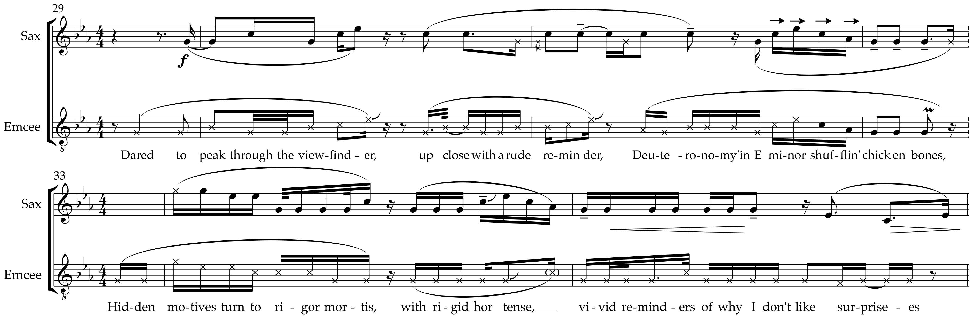
\includegraphics[width=\textwidth]{images/figures/chp 03/120137nonciphermimesis.pdf}
        \caption{Mimesis in R.A.P. Ferreira's ``NONCIPHER,'' 1:20--1:37.}
        \label{fig:rorymimesis}
    \end{figure}


Along with his persistent use of closing fragmentation noted above, another technique that manifests in his
musical performance is vocal mimesis of other elements of the texture. Figure~\ref{fig:rorymimesis} examines
instances in the second verse of ``NONCIPHER'' where Ferreira delivers his verse in mimetic dialogue with the
alto saxophone, live-tracked by Aaron Shaw. Following a verse that ends in closing fragmentation, Ferreira and
Shaw both anticipate m.~30 with syncopated entrances to the next section. Ferreira's first clause of text 
(``Dared to peak through the viewfinder'') aligns with Shaw's performance in both rhythmic placement and pitch 
contour. The first saxophone lick also informs his delivery of the next unit (``up close with a rude reminder'').
The most prominent moment of this first exchanges comes as Ferreira approaches the downbeat of m.~32: he sings
the phrase ``shufflin' chicken bones'' with the same melodic inflection as Shaw, adding a shake to his delivery
at the phrase's end.

After a brief departure from the mimicking the saxphone, Ferreira locks back in with Shaw at the onset of m.~34.
Traversing into a higher register to mimic the saxophone's G5, he raps ``[hidden] motives turn to rigor mortis,''
descending in relatino to but staggered from Shaw's C minor triad. The lick outlining G to C (m.~34, beat 2) that
Shaw delivers gives Ferreira another contour to mimic within the beats that immediately follow: ``rigid hortense''
ends with a shadow vowel that inflects upwards, and ``vivid reminders'' sounds its final syllable higher as well.
Ferreira approximates the saxophone's pitch and articulation through the beginning of this verse, mimicking Shaw's
performance.

The rhetorical value these instances relates to Ferreira's identity as an underground emcee. That he draws the
listener into the saxophone melody demonstrates his own musicality: he approaches performing his flow as a muiscal
participant. The beat in this section is not sounding around or behind his flow; instead, he performs his verse
\emph{as} a listener, encouraging a similar engagement \emph{from} the listener. As a result, the hierarchy between
beat and flow changes: the emcee's performance does not supersede any instrumental stream simply because of its use
of text. Instead, the text is fused to the music surrounding it.

%\clearpage
\phantomsection
\subsection*{\centering Moor Mother,  billy woods, and ELUCID's ``Tiberius''}
\addcontentsline{toc}{subsection}{Moor Mother, billy woods, and ELUCID's ``Tiberius''}

An underground emcee's fusion of text to music also informs the use of processing as a performance technique. Many 
are often responsible not only the construction and performance of their own text but often the means of capturing
their voice during the recording process. Although a quality microphone with some compression, EQ, and reverb works
sufficiently for many emcees, others, such as Moor Mother, explore a wider range of possibilities for what tracking
rap vocals entails. Her verse on the track ``Tiberius'' featuring ELUCID from \textit{Brass} (2020), her collaborative
LP with billy woods, illustrates her more maximal approach to fitting her voice in the musical texture.

Moor Mother's use of multitracking and effects processing demands a wider conception of the idea of a single ``vocal 
stream'' within the beat. Figure~\ref{fig:moormotherprocess} details the components of her vocal tracking in the 
first fifteen bars of her verse. Entering during the final bar ELUCID's verse, she repeats the text he just delivered
(``It's me dummy!'') transition to her own. The channel on which this verse enters (Moor Mother II in the figure) 
proves to be a secondary, ad-lib track, as a more-prominent vocal enters in the next bar (Moor Mother I in the figure).
This vocal channel bifurcates into a lower, primary layer of vocals and one created with a transposition effect, 
sounding around a fifth higher than the primary layer; the split is represented with normal and diamond head notation.

\begin{figure}[!p]
    \centering
    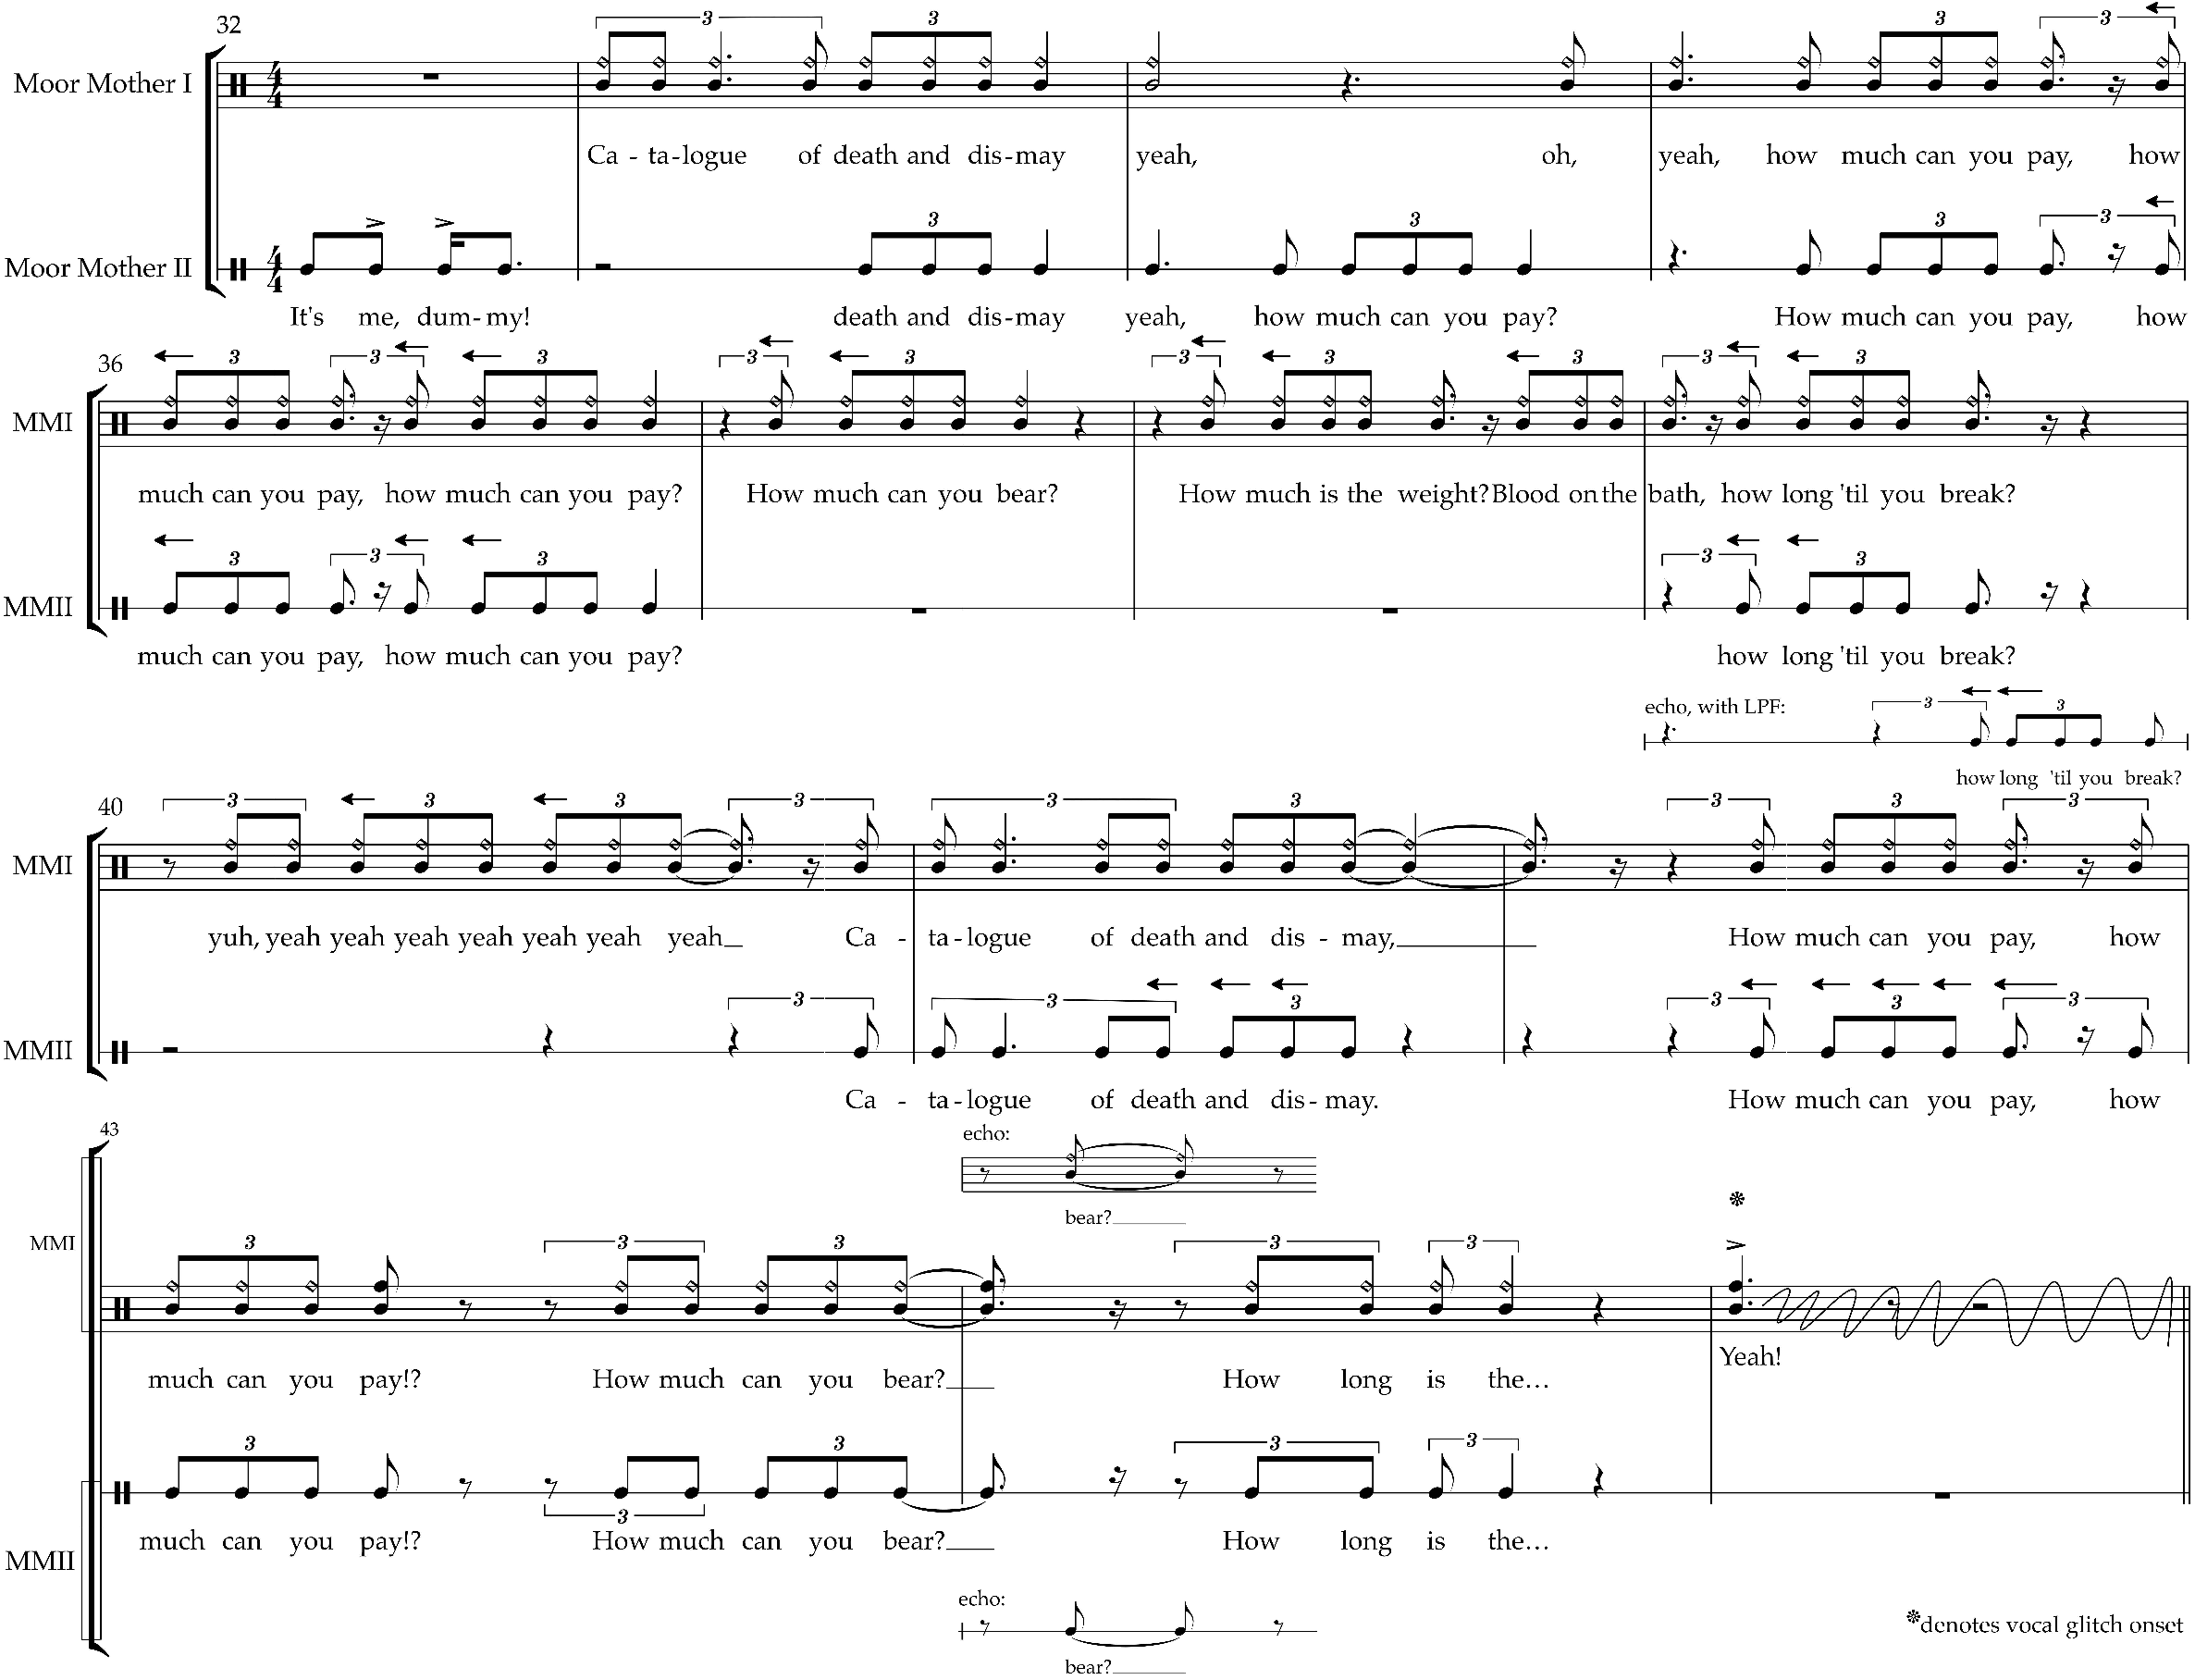
\includegraphics[width=\textwidth]{images/figures/chp 03/107136tiberiusprocessing.pdf}
    \caption{Vocal processing in Moor Mother and billy woods' ``Tiberius,'' 1:07--1:37.}
    \label{fig:moormotherprocess}
\end{figure}

Moor Mother uses these two vocal channels to deliver the first twelve bars of her verse: a series of questions rapped
in a triplet flow pattern that slightly anticipates the beat. The hurried, harsh delivery of her verse crests in mm. 
39--41, where she shifts the delivery far enough forward in the grove that the first eighth-note of her tuplet on the
text ``Catalogue of death and dismay'' syncopates before the downbeat. Prior to this rhythmic shift, she adds an echo
of the triplet ad-lib on ``how long `til you break,'' panned hard left in the mix and processed with a low-pass EQ
filter to diminish its prominence in the mix, shown in Figure~\ref{fig:moormotherprocess} on an ossia staff below Moor
Mother II.

In the next three measures, Moor Mother's use of processing signals a division within her verse\textemdash a transition
to a new flow and verse-part. Repeating text in a new rhythmic position, she arrives at the question ``How much can you 
bear?'' slightly before the downbeat of m.~44. Another echo repeats the text ``bear'' mid-measure, this time in both vocal
channels. Trailing off during the final question ``How long is the (wait),'' she delivers a guttural ``yeah!'' exclamation
on the downbeat.

This moment of transition is marked out with effects processing throughout the texture: the synth, which had dropped out
upon the textual repeat, now re-enters with a wash of noise while Moor Mother's textual exclamation is extended through
the use of a glitch-like delay. The delay used in this instance increases the frequency of signal repetitions at the same
time that it extends the feedback time for the loop, letting the sound of the ``Yeah!'' repeat more rapidly and extend
across the next two bars. This glitch is also foregrounded in the mix through the use of stereoscopic space: the delayed
signal ``ping-pongs'' back and forth between the right and left audio channels.

Once glitched, the function of the exclamation is no longer textual in the way any of the questions preceding it have been.
The transformed audio of Moor Mother's voice carries less semantic weight and functions more abstractly as sound, receding
into the mix as she begins the next section of her verse. Throughout the section, Moor Mother's treatment of her vocals
demonstrates that they take on multiple functions. Certainly, they carry the text, and the text carries semantic value, 
perhaps even poetic meaning for the listener. But the use of several distinct and overlapping vocal signals, each with its
own performative subtleties conceptually stratifies the concept of ``the vocals'' within the musical texture. Her particular
approach heightens the voice to become \emph{synthetic}; each layer's treatment could be likened to several oscillators used
to create a synthesizer patch. Rather than approaching vocal tracking as the creation of several contrapuntal lines, Moor
Mother's audio processing creates heterogeneity within a single ``line'' of music, likening the voice's role to any other
multitracked musical element in the mix.